% Created by tikzDevice version 0.12.3 on 2020-10-30 19:57:24
% !TEX encoding = UTF-8 Unicode
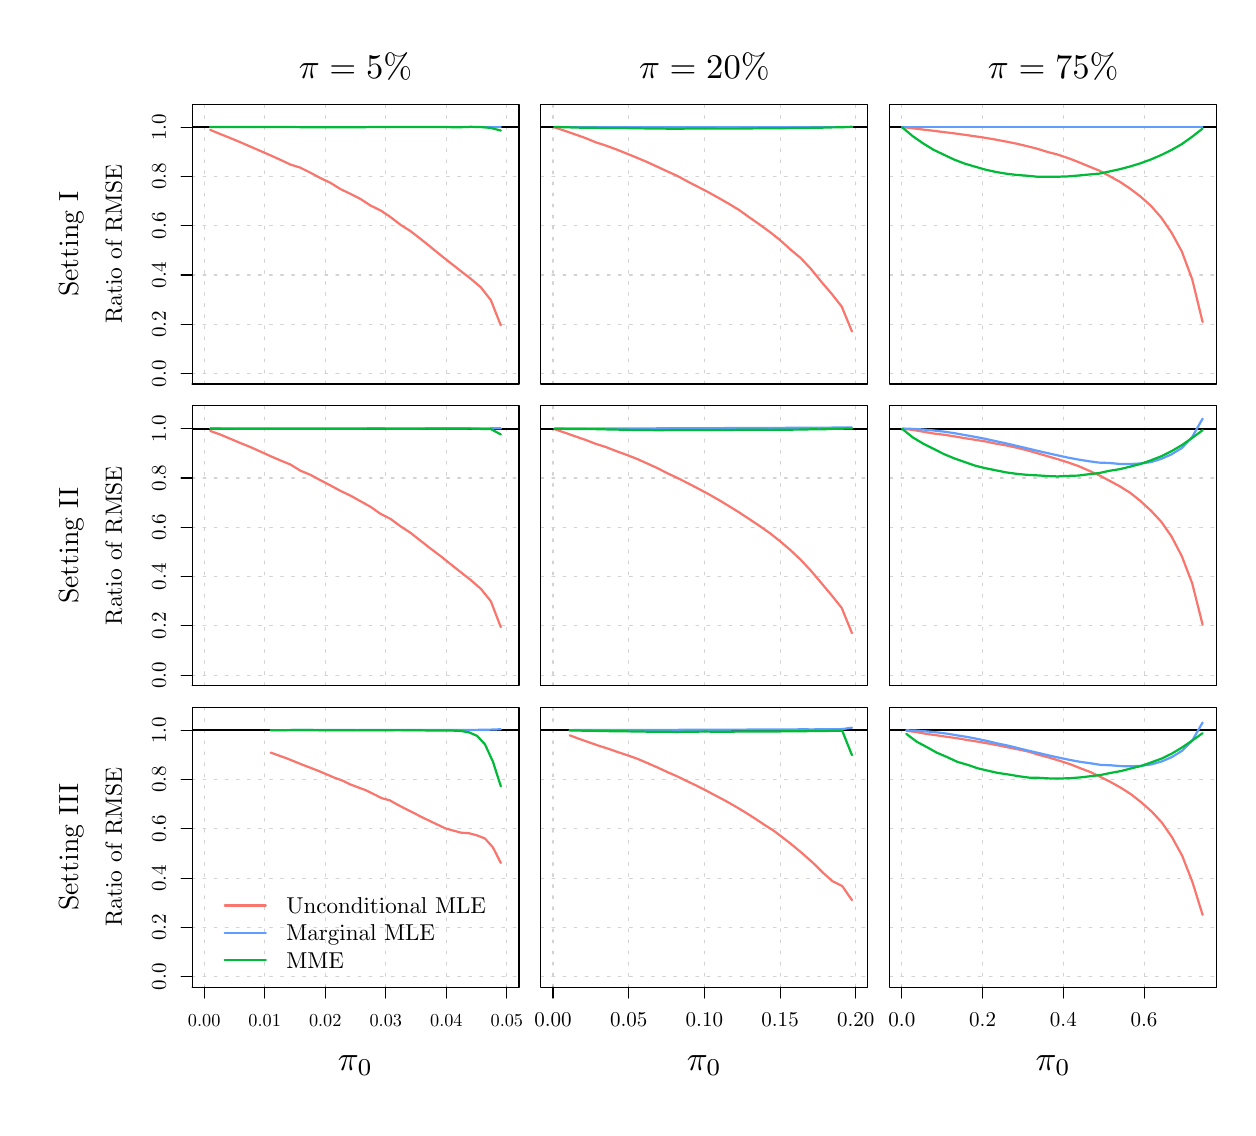
\begin{tikzpicture}[x=1pt,y=1pt]
\definecolor{fillColor}{RGB}{255,255,255}
\path[use as bounding box,fill=fillColor,fill opacity=0.00] (0,0) rectangle (433.62,390.26);
\begin{scope}
\path[clip] ( 55.44,257.53) rectangle (181.50,366.50);
\definecolor{drawColor}{RGB}{0,0,0}

\node[text=drawColor,anchor=base,inner sep=0pt, outer sep=0pt, scale=  0.66] at (118.47,231.40) {Simulation ID};

\node[text=drawColor,rotate= 90.00,anchor=base,inner sep=0pt, outer sep=0pt, scale=  0.66] at ( 34.06,312.01) {Ratio of RMSE};
\end{scope}
\begin{scope}
\path[clip] (  0.00,  0.00) rectangle (433.62,390.26);
\definecolor{drawColor}{RGB}{0,0,0}

\path[draw=drawColor,line width= 0.4pt,line join=round,line cap=round] ( 59.40,265.23) -- ( 59.40,354.34);

\path[draw=drawColor,line width= 0.4pt,line join=round,line cap=round] ( 59.40,265.23) -- ( 55.44,265.23);

\path[draw=drawColor,line width= 0.4pt,line join=round,line cap=round] ( 59.40,283.06) -- ( 55.44,283.06);

\path[draw=drawColor,line width= 0.4pt,line join=round,line cap=round] ( 59.40,300.88) -- ( 55.44,300.88);

\path[draw=drawColor,line width= 0.4pt,line join=round,line cap=round] ( 59.40,318.70) -- ( 55.44,318.70);

\path[draw=drawColor,line width= 0.4pt,line join=round,line cap=round] ( 59.40,336.52) -- ( 55.44,336.52);

\path[draw=drawColor,line width= 0.4pt,line join=round,line cap=round] ( 59.40,354.34) -- ( 55.44,354.34);

\node[text=drawColor,rotate= 90.00,anchor=base,inner sep=0pt, outer sep=0pt, scale=  0.76] at ( 49.90,265.23) {0.0};

\node[text=drawColor,rotate= 90.00,anchor=base,inner sep=0pt, outer sep=0pt, scale=  0.76] at ( 49.90,283.06) {0.2};

\node[text=drawColor,rotate= 90.00,anchor=base,inner sep=0pt, outer sep=0pt, scale=  0.76] at ( 49.90,300.88) {0.4};

\node[text=drawColor,rotate= 90.00,anchor=base,inner sep=0pt, outer sep=0pt, scale=  0.76] at ( 49.90,318.70) {0.6};

\node[text=drawColor,rotate= 90.00,anchor=base,inner sep=0pt, outer sep=0pt, scale=  0.76] at ( 49.90,336.52) {0.8};

\node[text=drawColor,rotate= 90.00,anchor=base,inner sep=0pt, outer sep=0pt, scale=  0.76] at ( 49.90,354.34) {1.0};
\end{scope}
\begin{scope}
\path[clip] ( 59.40,261.49) rectangle (177.54,362.54);
\definecolor{drawColor}{RGB}{211,211,211}

\path[draw=drawColor,line width= 0.4pt,dash pattern=on 1pt off 3pt ,line join=round,line cap=round] ( 63.78,261.49) -- ( 63.78,362.54);

\path[draw=drawColor,line width= 0.4pt,dash pattern=on 1pt off 3pt ,line join=round,line cap=round] ( 85.65,261.49) -- ( 85.65,362.54);

\path[draw=drawColor,line width= 0.4pt,dash pattern=on 1pt off 3pt ,line join=round,line cap=round] (107.53,261.49) -- (107.53,362.54);

\path[draw=drawColor,line width= 0.4pt,dash pattern=on 1pt off 3pt ,line join=round,line cap=round] (129.41,261.49) -- (129.41,362.54);

\path[draw=drawColor,line width= 0.4pt,dash pattern=on 1pt off 3pt ,line join=round,line cap=round] (151.29,261.49) -- (151.29,362.54);

\path[draw=drawColor,line width= 0.4pt,dash pattern=on 1pt off 3pt ,line join=round,line cap=round] (173.16,261.49) -- (173.16,362.54);

\path[draw=drawColor,line width= 0.4pt,dash pattern=on 1pt off 3pt ,line join=round,line cap=round] ( 59.40,265.23) -- (177.54,265.23);

\path[draw=drawColor,line width= 0.4pt,dash pattern=on 1pt off 3pt ,line join=round,line cap=round] ( 59.40,283.06) -- (177.54,283.06);

\path[draw=drawColor,line width= 0.4pt,dash pattern=on 1pt off 3pt ,line join=round,line cap=round] ( 59.40,300.88) -- (177.54,300.88);

\path[draw=drawColor,line width= 0.4pt,dash pattern=on 1pt off 3pt ,line join=round,line cap=round] ( 59.40,318.70) -- (177.54,318.70);

\path[draw=drawColor,line width= 0.4pt,dash pattern=on 1pt off 3pt ,line join=round,line cap=round] ( 59.40,336.52) -- (177.54,336.52);

\path[draw=drawColor,line width= 0.4pt,dash pattern=on 1pt off 3pt ,line join=round,line cap=round] ( 59.40,354.34) -- (177.54,354.34);
\end{scope}
\begin{scope}
\path[clip] (  0.00,  0.00) rectangle (433.62,390.26);
\definecolor{drawColor}{RGB}{0,0,0}

\path[draw=drawColor,line width= 0.4pt,line join=round,line cap=round] ( 59.40,261.49) --
	(177.54,261.49) --
	(177.54,362.54) --
	( 59.40,362.54) --
	( 59.40,261.49);
\end{scope}
\begin{scope}
\path[clip] ( 59.40,261.49) rectangle (177.54,362.54);
\definecolor{drawColor}{RGB}{0,0,0}

\path[draw=drawColor,line width= 0.8pt,line join=round,line cap=round] ( 59.40,354.34) -- (177.54,354.34);
\definecolor{drawColor}{RGB}{248,118,109}

\path[draw=drawColor,line width= 0.8pt,line join=round,line cap=round] ( 65.96,353.33) --
	( 69.58,351.82) --
	( 73.21,350.37) --
	( 76.83,348.87) --
	( 80.45,347.29) --
	( 84.07,345.72) --
	( 87.69,344.14) --
	( 91.31,342.51) --
	( 94.93,340.81) --
	( 98.55,339.66) --
	(102.17,337.85) --
	(105.80,335.90) --
	(109.42,334.19) --
	(113.04,331.91) --
	(116.66,330.20) --
	(120.28,328.34) --
	(123.90,325.98) --
	(127.52,324.22) --
	(131.14,321.79) --
	(134.77,319.00) --
	(138.39,316.70) --
	(142.01,313.90) --
	(145.63,310.99) --
	(149.25,308.03) --
	(152.87,305.17) --
	(156.49,302.32) --
	(160.11,299.53) --
	(163.73,296.45) --
	(167.36,291.81) --
	(170.98,282.65);
\definecolor{drawColor}{RGB}{97,156,255}

\path[draw=drawColor,line width= 0.8pt,line join=round,line cap=round] ( 65.96,354.34) --
	( 69.58,354.34) --
	( 73.21,354.34) --
	( 76.83,354.34) --
	( 80.45,354.34) --
	( 84.07,354.34) --
	( 87.69,354.34) --
	( 91.31,354.34) --
	( 94.93,354.34) --
	( 98.55,354.34) --
	(102.17,354.34) --
	(105.80,354.34) --
	(109.42,354.34) --
	(113.04,354.34) --
	(116.66,354.34) --
	(120.28,354.34) --
	(123.90,354.34) --
	(127.52,354.34) --
	(131.14,354.34) --
	(134.77,354.34) --
	(138.39,354.34) --
	(142.01,354.34) --
	(145.63,354.34) --
	(149.25,354.34) --
	(152.87,354.34) --
	(156.49,354.34) --
	(160.11,354.34) --
	(163.73,354.34) --
	(167.36,354.34) --
	(170.98,354.34);
\definecolor{drawColor}{RGB}{0,186,56}

\path[draw=drawColor,line width= 0.8pt,line join=round,line cap=round] ( 65.96,354.34) --
	( 69.58,354.34) --
	( 73.21,354.34) --
	( 76.83,354.36) --
	( 80.45,354.36) --
	( 84.07,354.35) --
	( 87.69,354.33) --
	( 91.31,354.33) --
	( 94.93,354.34) --
	( 98.55,354.31) --
	(102.17,354.30) --
	(105.80,354.29) --
	(109.42,354.27) --
	(113.04,354.28) --
	(116.66,354.27) --
	(120.28,354.29) --
	(123.90,354.33) --
	(127.52,354.35) --
	(131.14,354.37) --
	(134.77,354.37) --
	(138.39,354.34) --
	(142.01,354.35) --
	(145.63,354.40) --
	(149.25,354.39) --
	(152.87,354.31) --
	(156.49,354.29) --
	(160.11,354.43) --
	(163.73,354.34) --
	(167.36,354.03) --
	(170.98,353.08);
\end{scope}
\begin{scope}
\path[clip] (  0.00,  0.00) rectangle (433.62,390.26);
\definecolor{drawColor}{RGB}{0,0,0}

\node[text=drawColor,rotate= 90.00,anchor=base,inner sep=0pt, outer sep=0pt, scale=  1.00] at ( 18.22,312.01) {Setting I};

\node[text=drawColor,rotate= 90.00,anchor=base,inner sep=0pt, outer sep=0pt, scale=  0.85] at ( 34.06,312.01) {Ratio of RMSE};

\node[text=drawColor,anchor=base,inner sep=0pt, outer sep=0pt, scale=  1.25] at (118.47,372.04) {$\pi = 5\%$};
\end{scope}
\begin{scope}
\path[clip] (181.50,257.53) rectangle (307.56,366.50);
\definecolor{drawColor}{RGB}{0,0,0}

\node[text=drawColor,anchor=base,inner sep=0pt, outer sep=0pt, scale=  0.66] at (244.53,231.40) {Simulation ID};

\node[text=drawColor,rotate= 90.00,anchor=base,inner sep=0pt, outer sep=0pt, scale=  0.66] at (160.12,312.01) {Ratio of RMSE};
\end{scope}
\begin{scope}
\path[clip] (185.46,261.49) rectangle (303.60,362.54);
\definecolor{drawColor}{RGB}{211,211,211}

\path[draw=drawColor,line width= 0.4pt,dash pattern=on 1pt off 3pt ,line join=round,line cap=round] (189.84,261.49) -- (189.84,362.54);

\path[draw=drawColor,line width= 0.4pt,dash pattern=on 1pt off 3pt ,line join=round,line cap=round] (217.18,261.49) -- (217.18,362.54);

\path[draw=drawColor,line width= 0.4pt,dash pattern=on 1pt off 3pt ,line join=round,line cap=round] (244.53,261.49) -- (244.53,362.54);

\path[draw=drawColor,line width= 0.4pt,dash pattern=on 1pt off 3pt ,line join=round,line cap=round] (271.88,261.49) -- (271.88,362.54);

\path[draw=drawColor,line width= 0.4pt,dash pattern=on 1pt off 3pt ,line join=round,line cap=round] (299.22,261.49) -- (299.22,362.54);

\path[draw=drawColor,line width= 0.4pt,dash pattern=on 1pt off 3pt ,line join=round,line cap=round] (185.46,265.23) -- (303.60,265.23);

\path[draw=drawColor,line width= 0.4pt,dash pattern=on 1pt off 3pt ,line join=round,line cap=round] (185.46,283.06) -- (303.60,283.06);

\path[draw=drawColor,line width= 0.4pt,dash pattern=on 1pt off 3pt ,line join=round,line cap=round] (185.46,300.88) -- (303.60,300.88);

\path[draw=drawColor,line width= 0.4pt,dash pattern=on 1pt off 3pt ,line join=round,line cap=round] (185.46,318.70) -- (303.60,318.70);

\path[draw=drawColor,line width= 0.4pt,dash pattern=on 1pt off 3pt ,line join=round,line cap=round] (185.46,336.52) -- (303.60,336.52);

\path[draw=drawColor,line width= 0.4pt,dash pattern=on 1pt off 3pt ,line join=round,line cap=round] (185.46,354.34) -- (303.60,354.34);
\end{scope}
\begin{scope}
\path[clip] (  0.00,  0.00) rectangle (433.62,390.26);
\definecolor{drawColor}{RGB}{0,0,0}

\path[draw=drawColor,line width= 0.4pt,line join=round,line cap=round] (185.46,261.49) --
	(303.60,261.49) --
	(303.60,362.54) --
	(185.46,362.54) --
	(185.46,261.49);
\end{scope}
\begin{scope}
\path[clip] (185.46,261.49) rectangle (303.60,362.54);
\definecolor{drawColor}{RGB}{0,0,0}

\path[draw=drawColor,line width= 0.8pt,line join=round,line cap=round] (185.46,354.34) -- (303.60,354.34);
\definecolor{drawColor}{RGB}{248,118,109}

\path[draw=drawColor,line width= 0.8pt,line join=round,line cap=round] (190.38,354.23) --
	(194.09,353.00) --
	(197.79,351.70) --
	(201.50,350.40) --
	(205.21,348.86) --
	(208.91,347.66) --
	(212.62,346.30) --
	(216.32,344.82) --
	(220.03,343.31) --
	(223.74,341.74) --
	(227.44,340.04) --
	(231.15,338.31) --
	(234.85,336.65) --
	(238.56,334.62) --
	(242.27,332.71) --
	(245.97,330.80) --
	(249.68,328.72) --
	(253.38,326.61) --
	(257.09,324.36) --
	(260.80,321.69) --
	(264.50,319.11) --
	(268.21,316.41) --
	(271.91,313.47) --
	(275.62,310.11) --
	(279.33,307.02) --
	(283.03,303.08) --
	(286.74,298.50) --
	(290.45,294.17) --
	(294.15,289.48) --
	(297.86,280.46);
\definecolor{drawColor}{RGB}{97,156,255}

\path[draw=drawColor,line width= 0.8pt,line join=round,line cap=round] (190.38,354.34) --
	(194.09,354.34) --
	(197.79,354.34) --
	(201.50,354.34) --
	(205.21,354.34) --
	(208.91,354.34) --
	(212.62,354.34) --
	(216.32,354.34) --
	(220.03,354.34) --
	(223.74,354.34) --
	(227.44,354.34) --
	(231.15,354.34) --
	(234.85,354.34) --
	(238.56,354.34) --
	(242.27,354.34) --
	(245.97,354.34) --
	(249.68,354.34) --
	(253.38,354.34) --
	(257.09,354.34) --
	(260.80,354.34) --
	(264.50,354.34) --
	(268.21,354.34) --
	(271.91,354.34) --
	(275.62,354.34) --
	(279.33,354.34) --
	(283.03,354.34) --
	(286.74,354.34) --
	(290.45,354.34) --
	(294.15,354.34) --
	(297.86,354.34);
\definecolor{drawColor}{RGB}{0,186,56}

\path[draw=drawColor,line width= 0.8pt,line join=round,line cap=round] (190.38,354.38) --
	(194.09,354.29) --
	(197.79,354.17) --
	(201.50,354.07) --
	(205.21,354.06) --
	(208.91,354.01) --
	(212.62,353.97) --
	(216.32,353.98) --
	(220.03,353.89) --
	(223.74,353.85) --
	(227.44,353.83) --
	(231.15,353.76) --
	(234.85,353.73) --
	(238.56,353.79) --
	(242.27,353.83) --
	(245.97,353.81) --
	(249.68,353.77) --
	(253.38,353.78) --
	(257.09,353.78) --
	(260.80,353.85) --
	(264.50,353.88) --
	(268.21,353.92) --
	(271.91,353.92) --
	(275.62,353.97) --
	(279.33,353.97) --
	(283.03,354.06) --
	(286.74,354.11) --
	(290.45,354.22) --
	(294.15,354.26) --
	(297.86,354.45);
\end{scope}
\begin{scope}
\path[clip] (  0.00,  0.00) rectangle (433.62,390.26);
\definecolor{drawColor}{RGB}{0,0,0}

\node[text=drawColor,anchor=base,inner sep=0pt, outer sep=0pt, scale=  1.25] at (244.53,372.04) {$\pi = 20\%$};
\end{scope}
\begin{scope}
\path[clip] (307.56,257.53) rectangle (433.62,366.50);
\definecolor{drawColor}{RGB}{0,0,0}

\node[text=drawColor,anchor=base,inner sep=0pt, outer sep=0pt, scale=  0.66] at (370.59,231.40) {Simulation ID};

\node[text=drawColor,rotate= 90.00,anchor=base,inner sep=0pt, outer sep=0pt, scale=  0.66] at (286.18,312.01) {Ratio of RMSE};
\end{scope}
\begin{scope}
\path[clip] (311.52,261.49) rectangle (429.66,362.54);
\definecolor{drawColor}{RGB}{211,211,211}

\path[draw=drawColor,line width= 0.4pt,dash pattern=on 1pt off 3pt ,line join=round,line cap=round] (315.90,261.49) -- (315.90,362.54);

\path[draw=drawColor,line width= 0.4pt,dash pattern=on 1pt off 3pt ,line join=round,line cap=round] (345.07,261.49) -- (345.07,362.54);

\path[draw=drawColor,line width= 0.4pt,dash pattern=on 1pt off 3pt ,line join=round,line cap=round] (374.24,261.49) -- (374.24,362.54);

\path[draw=drawColor,line width= 0.4pt,dash pattern=on 1pt off 3pt ,line join=round,line cap=round] (403.41,261.49) -- (403.41,362.54);

\path[draw=drawColor,line width= 0.4pt,dash pattern=on 1pt off 3pt ,line join=round,line cap=round] (311.52,265.23) -- (429.66,265.23);

\path[draw=drawColor,line width= 0.4pt,dash pattern=on 1pt off 3pt ,line join=round,line cap=round] (311.52,283.06) -- (429.66,283.06);

\path[draw=drawColor,line width= 0.4pt,dash pattern=on 1pt off 3pt ,line join=round,line cap=round] (311.52,300.88) -- (429.66,300.88);

\path[draw=drawColor,line width= 0.4pt,dash pattern=on 1pt off 3pt ,line join=round,line cap=round] (311.52,318.70) -- (429.66,318.70);

\path[draw=drawColor,line width= 0.4pt,dash pattern=on 1pt off 3pt ,line join=round,line cap=round] (311.52,336.52) -- (429.66,336.52);

\path[draw=drawColor,line width= 0.4pt,dash pattern=on 1pt off 3pt ,line join=round,line cap=round] (311.52,354.34) -- (429.66,354.34);
\end{scope}
\begin{scope}
\path[clip] (  0.00,  0.00) rectangle (433.62,390.26);
\definecolor{drawColor}{RGB}{0,0,0}

\path[draw=drawColor,line width= 0.4pt,line join=round,line cap=round] (311.52,261.49) --
	(429.66,261.49) --
	(429.66,362.54) --
	(311.52,362.54) --
	(311.52,261.49);
\end{scope}
\begin{scope}
\path[clip] (311.52,261.49) rectangle (429.66,362.54);
\definecolor{drawColor}{RGB}{0,0,0}

\path[draw=drawColor,line width= 0.8pt,line join=round,line cap=round] (311.52,354.34) -- (429.66,354.34);
\definecolor{drawColor}{RGB}{248,118,109}

\path[draw=drawColor,line width= 0.8pt,line join=round,line cap=round] (316.04,354.34) --
	(319.78,353.91) --
	(323.53,353.44) --
	(327.27,353.01) --
	(331.01,352.52) --
	(334.75,352.08) --
	(338.49,351.56) --
	(342.23,351.02) --
	(345.98,350.46) --
	(349.72,349.82) --
	(353.46,349.11) --
	(357.20,348.37) --
	(360.94,347.48) --
	(364.69,346.54) --
	(368.43,345.37) --
	(372.17,344.41) --
	(375.91,343.16) --
	(379.65,341.71) --
	(383.39,340.16) --
	(387.14,338.64) --
	(390.88,336.66) --
	(394.62,334.58) --
	(398.36,332.09) --
	(402.10,329.26) --
	(405.85,325.91) --
	(409.59,321.66) --
	(413.33,316.20) --
	(417.07,309.33) --
	(420.81,299.28) --
	(424.56,283.89);
\definecolor{drawColor}{RGB}{97,156,255}

\path[draw=drawColor,line width= 0.8pt,line join=round,line cap=round] (316.04,354.34) --
	(319.78,354.34) --
	(323.53,354.34) --
	(327.27,354.34) --
	(331.01,354.34) --
	(334.75,354.34) --
	(338.49,354.34) --
	(342.23,354.34) --
	(345.98,354.34) --
	(349.72,354.34) --
	(353.46,354.34) --
	(357.20,354.34) --
	(360.94,354.34) --
	(364.69,354.34) --
	(368.43,354.34) --
	(372.17,354.34) --
	(375.91,354.34) --
	(379.65,354.34) --
	(383.39,354.34) --
	(387.14,354.34) --
	(390.88,354.34) --
	(394.62,354.34) --
	(398.36,354.34) --
	(402.10,354.34) --
	(405.85,354.34) --
	(409.59,354.34) --
	(413.33,354.34) --
	(417.07,354.34) --
	(420.81,354.34) --
	(424.56,354.34);
\definecolor{drawColor}{RGB}{0,186,56}

\path[draw=drawColor,line width= 0.8pt,line join=round,line cap=round] (316.04,354.24) --
	(319.78,351.07) --
	(323.53,348.47) --
	(327.27,346.16) --
	(331.01,344.37) --
	(334.75,342.60) --
	(338.49,341.17) --
	(342.23,340.06) --
	(345.98,338.98) --
	(349.72,338.15) --
	(353.46,337.51) --
	(357.20,337.06) --
	(360.94,336.77) --
	(364.69,336.41) --
	(368.43,336.40) --
	(372.17,336.39) --
	(375.91,336.52) --
	(379.65,336.83) --
	(383.39,337.19) --
	(387.14,337.51) --
	(390.88,338.29) --
	(394.62,339.11) --
	(398.36,340.10) --
	(402.10,341.25) --
	(405.85,342.62) --
	(409.59,344.24) --
	(413.33,346.08) --
	(417.07,348.21) --
	(420.81,350.87) --
	(424.56,353.81);
\end{scope}
\begin{scope}
\path[clip] (  0.00,  0.00) rectangle (433.62,390.26);
\definecolor{drawColor}{RGB}{0,0,0}

\node[text=drawColor,anchor=base,inner sep=0pt, outer sep=0pt, scale=  1.25] at (370.59,372.04) {$\pi = 75\%$};
\end{scope}
\begin{scope}
\path[clip] ( 55.44,148.57) rectangle (181.50,257.53);
\definecolor{drawColor}{RGB}{0,0,0}

\node[text=drawColor,anchor=base,inner sep=0pt, outer sep=0pt, scale=  0.66] at (118.47,122.43) {Simulation ID};

\node[text=drawColor,rotate= 90.00,anchor=base,inner sep=0pt, outer sep=0pt, scale=  0.66] at ( 34.06,203.05) {Ratio of RMSE};
\end{scope}
\begin{scope}
\path[clip] (  0.00,  0.00) rectangle (433.62,390.26);
\definecolor{drawColor}{RGB}{0,0,0}

\path[draw=drawColor,line width= 0.4pt,line join=round,line cap=round] ( 59.40,156.27) -- ( 59.40,245.37);

\path[draw=drawColor,line width= 0.4pt,line join=round,line cap=round] ( 59.40,156.27) -- ( 55.44,156.27);

\path[draw=drawColor,line width= 0.4pt,line join=round,line cap=round] ( 59.40,174.09) -- ( 55.44,174.09);

\path[draw=drawColor,line width= 0.4pt,line join=round,line cap=round] ( 59.40,191.91) -- ( 55.44,191.91);

\path[draw=drawColor,line width= 0.4pt,line join=round,line cap=round] ( 59.40,209.73) -- ( 55.44,209.73);

\path[draw=drawColor,line width= 0.4pt,line join=round,line cap=round] ( 59.40,227.55) -- ( 55.44,227.55);

\path[draw=drawColor,line width= 0.4pt,line join=round,line cap=round] ( 59.40,245.37) -- ( 55.44,245.37);

\node[text=drawColor,rotate= 90.00,anchor=base,inner sep=0pt, outer sep=0pt, scale=  0.76] at ( 49.90,156.27) {0.0};

\node[text=drawColor,rotate= 90.00,anchor=base,inner sep=0pt, outer sep=0pt, scale=  0.76] at ( 49.90,174.09) {0.2};

\node[text=drawColor,rotate= 90.00,anchor=base,inner sep=0pt, outer sep=0pt, scale=  0.76] at ( 49.90,191.91) {0.4};

\node[text=drawColor,rotate= 90.00,anchor=base,inner sep=0pt, outer sep=0pt, scale=  0.76] at ( 49.90,209.73) {0.6};

\node[text=drawColor,rotate= 90.00,anchor=base,inner sep=0pt, outer sep=0pt, scale=  0.76] at ( 49.90,227.55) {0.8};

\node[text=drawColor,rotate= 90.00,anchor=base,inner sep=0pt, outer sep=0pt, scale=  0.76] at ( 49.90,245.37) {1.0};
\end{scope}
\begin{scope}
\path[clip] ( 59.40,152.53) rectangle (177.54,253.57);
\definecolor{drawColor}{RGB}{211,211,211}

\path[draw=drawColor,line width= 0.4pt,dash pattern=on 1pt off 3pt ,line join=round,line cap=round] ( 63.78,152.53) -- ( 63.78,253.57);

\path[draw=drawColor,line width= 0.4pt,dash pattern=on 1pt off 3pt ,line join=round,line cap=round] ( 85.65,152.53) -- ( 85.65,253.57);

\path[draw=drawColor,line width= 0.4pt,dash pattern=on 1pt off 3pt ,line join=round,line cap=round] (107.53,152.53) -- (107.53,253.57);

\path[draw=drawColor,line width= 0.4pt,dash pattern=on 1pt off 3pt ,line join=round,line cap=round] (129.41,152.53) -- (129.41,253.57);

\path[draw=drawColor,line width= 0.4pt,dash pattern=on 1pt off 3pt ,line join=round,line cap=round] (151.29,152.53) -- (151.29,253.57);

\path[draw=drawColor,line width= 0.4pt,dash pattern=on 1pt off 3pt ,line join=round,line cap=round] (173.16,152.53) -- (173.16,253.57);

\path[draw=drawColor,line width= 0.4pt,dash pattern=on 1pt off 3pt ,line join=round,line cap=round] ( 59.40,156.27) -- (177.54,156.27);

\path[draw=drawColor,line width= 0.4pt,dash pattern=on 1pt off 3pt ,line join=round,line cap=round] ( 59.40,174.09) -- (177.54,174.09);

\path[draw=drawColor,line width= 0.4pt,dash pattern=on 1pt off 3pt ,line join=round,line cap=round] ( 59.40,191.91) -- (177.54,191.91);

\path[draw=drawColor,line width= 0.4pt,dash pattern=on 1pt off 3pt ,line join=round,line cap=round] ( 59.40,209.73) -- (177.54,209.73);

\path[draw=drawColor,line width= 0.4pt,dash pattern=on 1pt off 3pt ,line join=round,line cap=round] ( 59.40,227.55) -- (177.54,227.55);

\path[draw=drawColor,line width= 0.4pt,dash pattern=on 1pt off 3pt ,line join=round,line cap=round] ( 59.40,245.37) -- (177.54,245.37);
\end{scope}
\begin{scope}
\path[clip] (  0.00,  0.00) rectangle (433.62,390.26);
\definecolor{drawColor}{RGB}{0,0,0}

\path[draw=drawColor,line width= 0.4pt,line join=round,line cap=round] ( 59.40,152.53) --
	(177.54,152.53) --
	(177.54,253.57) --
	( 59.40,253.57) --
	( 59.40,152.53);
\end{scope}
\begin{scope}
\path[clip] ( 59.40,152.53) rectangle (177.54,253.57);
\definecolor{drawColor}{RGB}{0,0,0}

\path[draw=drawColor,line width= 0.8pt,line join=round,line cap=round] ( 59.40,245.37) -- (177.54,245.37);
\definecolor{drawColor}{RGB}{248,118,109}

\path[draw=drawColor,line width= 0.8pt,line join=round,line cap=round] ( 65.96,244.54) --
	( 69.58,243.24) --
	( 73.21,241.71) --
	( 76.83,240.18) --
	( 80.45,238.72) --
	( 84.07,237.10) --
	( 87.69,235.45) --
	( 91.31,233.89) --
	( 94.93,232.41) --
	( 98.55,230.18) --
	(102.17,228.68) --
	(105.80,226.71) --
	(109.42,224.84) --
	(113.04,222.87) --
	(116.66,221.15) --
	(120.28,219.13) --
	(123.90,217.12) --
	(127.52,214.57) --
	(131.14,212.74) --
	(134.77,210.05) --
	(138.39,207.69) --
	(142.01,204.83) --
	(145.63,201.99) --
	(149.25,199.28) --
	(152.87,196.36) --
	(156.49,193.50) --
	(160.11,190.65) --
	(163.73,187.51) --
	(167.36,183.01) --
	(170.98,173.60);
\definecolor{drawColor}{RGB}{97,156,255}

\path[draw=drawColor,line width= 0.8pt,line join=round,line cap=round] ( 65.96,245.38) --
	( 69.58,245.38) --
	( 73.21,245.38) --
	( 76.83,245.39) --
	( 80.45,245.39) --
	( 84.07,245.39) --
	( 87.69,245.39) --
	( 91.31,245.40) --
	( 94.93,245.40) --
	( 98.55,245.40) --
	(102.17,245.41) --
	(105.80,245.41) --
	(109.42,245.41) --
	(113.04,245.42) --
	(116.66,245.42) --
	(120.28,245.42) --
	(123.90,245.42) --
	(127.52,245.42) --
	(131.14,245.43) --
	(134.77,245.44) --
	(138.39,245.43) --
	(142.01,245.44) --
	(145.63,245.44) --
	(149.25,245.44) --
	(152.87,245.45) --
	(156.49,245.45) --
	(160.11,245.46) --
	(163.73,245.46) --
	(167.36,245.47) --
	(170.98,245.48);
\definecolor{drawColor}{RGB}{0,186,56}

\path[draw=drawColor,line width= 0.8pt,line join=round,line cap=round] ( 65.96,245.39) --
	( 69.58,245.38) --
	( 73.21,245.37) --
	( 76.83,245.36) --
	( 80.45,245.35) --
	( 84.07,245.35) --
	( 87.69,245.35) --
	( 91.31,245.34) --
	( 94.93,245.33) --
	( 98.55,245.36) --
	(102.17,245.35) --
	(105.80,245.34) --
	(109.42,245.32) --
	(113.04,245.32) --
	(116.66,245.33) --
	(120.28,245.36) --
	(123.90,245.39) --
	(127.52,245.40) --
	(131.14,245.35) --
	(134.77,245.34) --
	(138.39,245.34) --
	(142.01,245.37) --
	(145.63,245.39) --
	(149.25,245.42) --
	(152.87,245.43) --
	(156.49,245.38) --
	(160.11,245.38) --
	(163.73,245.27) --
	(167.36,245.22) --
	(170.98,243.26);
\end{scope}
\begin{scope}
\path[clip] (  0.00,  0.00) rectangle (433.62,390.26);
\definecolor{drawColor}{RGB}{0,0,0}

\node[text=drawColor,rotate= 90.00,anchor=base,inner sep=0pt, outer sep=0pt, scale=  1.00] at ( 18.22,203.05) {Setting II};

\node[text=drawColor,rotate= 90.00,anchor=base,inner sep=0pt, outer sep=0pt, scale=  0.85] at ( 34.06,203.05) {Ratio of RMSE};
\end{scope}
\begin{scope}
\path[clip] (181.50,148.57) rectangle (307.56,257.53);
\definecolor{drawColor}{RGB}{0,0,0}

\node[text=drawColor,anchor=base,inner sep=0pt, outer sep=0pt, scale=  0.66] at (244.53,122.43) {Simulation ID};

\node[text=drawColor,rotate= 90.00,anchor=base,inner sep=0pt, outer sep=0pt, scale=  0.66] at (160.12,203.05) {Ratio of RMSE};
\end{scope}
\begin{scope}
\path[clip] (185.46,152.53) rectangle (303.60,253.57);
\definecolor{drawColor}{RGB}{211,211,211}

\path[draw=drawColor,line width= 0.4pt,dash pattern=on 1pt off 3pt ,line join=round,line cap=round] (189.84,152.53) -- (189.84,253.57);

\path[draw=drawColor,line width= 0.4pt,dash pattern=on 1pt off 3pt ,line join=round,line cap=round] (217.18,152.53) -- (217.18,253.57);

\path[draw=drawColor,line width= 0.4pt,dash pattern=on 1pt off 3pt ,line join=round,line cap=round] (244.53,152.53) -- (244.53,253.57);

\path[draw=drawColor,line width= 0.4pt,dash pattern=on 1pt off 3pt ,line join=round,line cap=round] (271.88,152.53) -- (271.88,253.57);

\path[draw=drawColor,line width= 0.4pt,dash pattern=on 1pt off 3pt ,line join=round,line cap=round] (299.22,152.53) -- (299.22,253.57);

\path[draw=drawColor,line width= 0.4pt,dash pattern=on 1pt off 3pt ,line join=round,line cap=round] (185.46,156.27) -- (303.60,156.27);

\path[draw=drawColor,line width= 0.4pt,dash pattern=on 1pt off 3pt ,line join=round,line cap=round] (185.46,174.09) -- (303.60,174.09);

\path[draw=drawColor,line width= 0.4pt,dash pattern=on 1pt off 3pt ,line join=round,line cap=round] (185.46,191.91) -- (303.60,191.91);

\path[draw=drawColor,line width= 0.4pt,dash pattern=on 1pt off 3pt ,line join=round,line cap=round] (185.46,209.73) -- (303.60,209.73);

\path[draw=drawColor,line width= 0.4pt,dash pattern=on 1pt off 3pt ,line join=round,line cap=round] (185.46,227.55) -- (303.60,227.55);

\path[draw=drawColor,line width= 0.4pt,dash pattern=on 1pt off 3pt ,line join=round,line cap=round] (185.46,245.37) -- (303.60,245.37);
\end{scope}
\begin{scope}
\path[clip] (  0.00,  0.00) rectangle (433.62,390.26);
\definecolor{drawColor}{RGB}{0,0,0}

\path[draw=drawColor,line width= 0.4pt,line join=round,line cap=round] (185.46,152.53) --
	(303.60,152.53) --
	(303.60,253.57) --
	(185.46,253.57) --
	(185.46,152.53);
\end{scope}
\begin{scope}
\path[clip] (185.46,152.53) rectangle (303.60,253.57);
\definecolor{drawColor}{RGB}{0,0,0}

\path[draw=drawColor,line width= 0.8pt,line join=round,line cap=round] (185.46,245.37) -- (303.60,245.37);
\definecolor{drawColor}{RGB}{248,118,109}

\path[draw=drawColor,line width= 0.8pt,line join=round,line cap=round] (190.38,245.18) --
	(194.09,243.93) --
	(197.79,242.59) --
	(201.50,241.33) --
	(205.21,239.89) --
	(208.91,238.73) --
	(212.62,237.27) --
	(216.32,235.94) --
	(220.03,234.49) --
	(223.74,232.84) --
	(227.44,231.15) --
	(231.15,229.25) --
	(234.85,227.52) --
	(238.56,225.65) --
	(242.27,223.71) --
	(245.97,221.75) --
	(249.68,219.63) --
	(253.38,217.40) --
	(257.09,215.09) --
	(260.80,212.66) --
	(264.50,210.19) --
	(268.21,207.59) --
	(271.91,204.65) --
	(275.62,201.48) --
	(279.33,197.98) --
	(283.03,194.02) --
	(286.74,189.64) --
	(290.45,185.21) --
	(294.15,180.58) --
	(297.86,171.46);
\definecolor{drawColor}{RGB}{97,156,255}

\path[draw=drawColor,line width= 0.8pt,line join=round,line cap=round] (190.38,245.38) --
	(194.09,245.39) --
	(197.79,245.40) --
	(201.50,245.41) --
	(205.21,245.42) --
	(208.91,245.43) --
	(212.62,245.44) --
	(216.32,245.44) --
	(220.03,245.45) --
	(223.74,245.46) --
	(227.44,245.47) --
	(231.15,245.47) --
	(234.85,245.49) --
	(238.56,245.50) --
	(242.27,245.52) --
	(245.97,245.53) --
	(249.68,245.55) --
	(253.38,245.57) --
	(257.09,245.58) --
	(260.80,245.60) --
	(264.50,245.60) --
	(268.21,245.62) --
	(271.91,245.64) --
	(275.62,245.66) --
	(279.33,245.66) --
	(283.03,245.68) --
	(286.74,245.73) --
	(290.45,245.74) --
	(294.15,245.77) --
	(297.86,245.82);
\definecolor{drawColor}{RGB}{0,186,56}

\path[draw=drawColor,line width= 0.8pt,line join=round,line cap=round] (190.38,245.35) --
	(194.09,245.28) --
	(197.79,245.24) --
	(201.50,245.20) --
	(205.21,245.19) --
	(208.91,245.10) --
	(212.62,245.03) --
	(216.32,244.94) --
	(220.03,244.89) --
	(223.74,244.86) --
	(227.44,244.81) --
	(231.15,244.83) --
	(234.85,244.88) --
	(238.56,244.88) --
	(242.27,244.88) --
	(245.97,244.85) --
	(249.68,244.85) --
	(253.38,244.89) --
	(257.09,244.94) --
	(260.80,244.95) --
	(264.50,244.97) --
	(268.21,244.92) --
	(271.91,244.99) --
	(275.62,245.00) --
	(279.33,245.02) --
	(283.03,245.12) --
	(286.74,245.10) --
	(290.45,245.27) --
	(294.15,245.35) --
	(297.86,245.44);
\end{scope}
\begin{scope}
\path[clip] (307.56,148.57) rectangle (433.62,257.53);
\definecolor{drawColor}{RGB}{0,0,0}

\node[text=drawColor,anchor=base,inner sep=0pt, outer sep=0pt, scale=  0.66] at (370.59,122.43) {Simulation ID};

\node[text=drawColor,rotate= 90.00,anchor=base,inner sep=0pt, outer sep=0pt, scale=  0.66] at (286.18,203.05) {Ratio of RMSE};
\end{scope}
\begin{scope}
\path[clip] (311.52,152.53) rectangle (429.66,253.57);
\definecolor{drawColor}{RGB}{211,211,211}

\path[draw=drawColor,line width= 0.4pt,dash pattern=on 1pt off 3pt ,line join=round,line cap=round] (315.90,152.53) -- (315.90,253.57);

\path[draw=drawColor,line width= 0.4pt,dash pattern=on 1pt off 3pt ,line join=round,line cap=round] (345.07,152.53) -- (345.07,253.57);

\path[draw=drawColor,line width= 0.4pt,dash pattern=on 1pt off 3pt ,line join=round,line cap=round] (374.24,152.53) -- (374.24,253.57);

\path[draw=drawColor,line width= 0.4pt,dash pattern=on 1pt off 3pt ,line join=round,line cap=round] (403.41,152.53) -- (403.41,253.57);

\path[draw=drawColor,line width= 0.4pt,dash pattern=on 1pt off 3pt ,line join=round,line cap=round] (311.52,156.27) -- (429.66,156.27);

\path[draw=drawColor,line width= 0.4pt,dash pattern=on 1pt off 3pt ,line join=round,line cap=round] (311.52,174.09) -- (429.66,174.09);

\path[draw=drawColor,line width= 0.4pt,dash pattern=on 1pt off 3pt ,line join=round,line cap=round] (311.52,191.91) -- (429.66,191.91);

\path[draw=drawColor,line width= 0.4pt,dash pattern=on 1pt off 3pt ,line join=round,line cap=round] (311.52,209.73) -- (429.66,209.73);

\path[draw=drawColor,line width= 0.4pt,dash pattern=on 1pt off 3pt ,line join=round,line cap=round] (311.52,227.55) -- (429.66,227.55);

\path[draw=drawColor,line width= 0.4pt,dash pattern=on 1pt off 3pt ,line join=round,line cap=round] (311.52,245.37) -- (429.66,245.37);
\end{scope}
\begin{scope}
\path[clip] (  0.00,  0.00) rectangle (433.62,390.26);
\definecolor{drawColor}{RGB}{0,0,0}

\path[draw=drawColor,line width= 0.4pt,line join=round,line cap=round] (311.52,152.53) --
	(429.66,152.53) --
	(429.66,253.57) --
	(311.52,253.57) --
	(311.52,152.53);
\end{scope}
\begin{scope}
\path[clip] (311.52,152.53) rectangle (429.66,253.57);
\definecolor{drawColor}{RGB}{0,0,0}

\path[draw=drawColor,line width= 0.8pt,line join=round,line cap=round] (311.52,245.37) -- (429.66,245.37);
\definecolor{drawColor}{RGB}{248,118,109}

\path[draw=drawColor,line width= 0.8pt,line join=round,line cap=round] (316.04,245.36) --
	(319.78,244.91) --
	(323.53,244.28) --
	(327.27,243.62) --
	(331.01,243.18) --
	(334.75,242.59) --
	(338.49,241.94) --
	(342.23,241.36) --
	(345.98,240.77) --
	(349.72,239.98) --
	(353.46,239.32) --
	(357.20,238.52) --
	(360.94,237.59) --
	(364.69,236.53) --
	(368.43,235.43) --
	(372.17,234.35) --
	(375.91,233.17) --
	(379.65,231.86) --
	(383.39,230.22) --
	(387.14,228.54) --
	(390.88,226.56) --
	(394.62,224.53) --
	(398.36,222.20) --
	(402.10,219.22) --
	(405.85,215.77) --
	(409.59,211.76) --
	(413.33,206.40) --
	(417.07,199.23) --
	(420.81,189.43) --
	(424.56,174.54);
\definecolor{drawColor}{RGB}{97,156,255}

\path[draw=drawColor,line width= 0.8pt,line join=round,line cap=round] (316.04,245.37) --
	(319.78,245.28) --
	(323.53,245.06) --
	(327.27,244.71) --
	(331.01,244.30) --
	(334.75,243.75) --
	(338.49,243.08) --
	(342.23,242.41) --
	(345.98,241.70) --
	(349.72,240.86) --
	(353.46,240.06) --
	(357.20,239.18) --
	(360.94,238.31) --
	(364.69,237.40) --
	(368.43,236.55) --
	(372.17,235.71) --
	(375.91,234.90) --
	(379.65,234.20) --
	(383.39,233.60) --
	(387.14,233.09) --
	(390.88,232.96) --
	(394.62,232.61) --
	(398.36,232.57) --
	(402.10,232.79) --
	(405.85,233.27) --
	(409.59,234.44) --
	(413.33,236.09) --
	(417.07,238.38) --
	(420.81,242.38) --
	(424.56,248.97);
\definecolor{drawColor}{RGB}{0,186,56}

\path[draw=drawColor,line width= 0.8pt,line join=round,line cap=round] (316.04,245.27) --
	(319.78,242.23) --
	(323.53,239.98) --
	(327.27,238.09) --
	(331.01,236.21) --
	(334.75,234.65) --
	(338.49,233.34) --
	(342.23,232.03) --
	(345.98,231.09) --
	(349.72,230.34) --
	(353.46,229.57) --
	(357.20,229.06) --
	(360.94,228.69) --
	(364.69,228.49) --
	(368.43,228.24) --
	(372.17,228.10) --
	(375.91,228.29) --
	(379.65,228.41) --
	(383.39,228.89) --
	(387.14,229.31) --
	(390.88,230.14) --
	(394.62,230.72) --
	(398.36,231.63) --
	(402.10,232.58) --
	(405.85,233.92) --
	(409.59,235.37) --
	(413.33,237.22) --
	(417.07,239.42) --
	(420.81,242.03) --
	(424.56,244.81);
\end{scope}
\begin{scope}
\path[clip] ( 55.44, 39.60) rectangle (181.50,148.57);
\definecolor{drawColor}{RGB}{0,0,0}

\node[text=drawColor,anchor=base,inner sep=0pt, outer sep=0pt, scale=  0.66] at (118.47, 13.46) {Simulation ID};

\node[text=drawColor,rotate= 90.00,anchor=base,inner sep=0pt, outer sep=0pt, scale=  0.66] at ( 34.06, 94.08) {Ratio of RMSE};
\end{scope}
\begin{scope}
\path[clip] (  0.00,  0.00) rectangle (433.62,390.26);
\definecolor{drawColor}{RGB}{0,0,0}

\path[draw=drawColor,line width= 0.4pt,line join=round,line cap=round] ( 59.40, 47.30) -- ( 59.40,136.41);

\path[draw=drawColor,line width= 0.4pt,line join=round,line cap=round] ( 59.40, 47.30) -- ( 55.44, 47.30);

\path[draw=drawColor,line width= 0.4pt,line join=round,line cap=round] ( 59.40, 65.12) -- ( 55.44, 65.12);

\path[draw=drawColor,line width= 0.4pt,line join=round,line cap=round] ( 59.40, 82.94) -- ( 55.44, 82.94);

\path[draw=drawColor,line width= 0.4pt,line join=round,line cap=round] ( 59.40,100.77) -- ( 55.44,100.77);

\path[draw=drawColor,line width= 0.4pt,line join=round,line cap=round] ( 59.40,118.59) -- ( 55.44,118.59);

\path[draw=drawColor,line width= 0.4pt,line join=round,line cap=round] ( 59.40,136.41) -- ( 55.44,136.41);

\node[text=drawColor,rotate= 90.00,anchor=base,inner sep=0pt, outer sep=0pt, scale=  0.76] at ( 49.90, 47.30) {0.0};

\node[text=drawColor,rotate= 90.00,anchor=base,inner sep=0pt, outer sep=0pt, scale=  0.76] at ( 49.90, 65.12) {0.2};

\node[text=drawColor,rotate= 90.00,anchor=base,inner sep=0pt, outer sep=0pt, scale=  0.76] at ( 49.90, 82.94) {0.4};

\node[text=drawColor,rotate= 90.00,anchor=base,inner sep=0pt, outer sep=0pt, scale=  0.76] at ( 49.90,100.77) {0.6};

\node[text=drawColor,rotate= 90.00,anchor=base,inner sep=0pt, outer sep=0pt, scale=  0.76] at ( 49.90,118.59) {0.8};

\node[text=drawColor,rotate= 90.00,anchor=base,inner sep=0pt, outer sep=0pt, scale=  0.76] at ( 49.90,136.41) {1.0};
\end{scope}
\begin{scope}
\path[clip] ( 59.40, 43.56) rectangle (177.54,144.61);
\definecolor{drawColor}{RGB}{211,211,211}

\path[draw=drawColor,line width= 0.4pt,dash pattern=on 1pt off 3pt ,line join=round,line cap=round] ( 63.78, 43.56) -- ( 63.78,144.61);

\path[draw=drawColor,line width= 0.4pt,dash pattern=on 1pt off 3pt ,line join=round,line cap=round] ( 85.65, 43.56) -- ( 85.65,144.61);

\path[draw=drawColor,line width= 0.4pt,dash pattern=on 1pt off 3pt ,line join=round,line cap=round] (107.53, 43.56) -- (107.53,144.61);

\path[draw=drawColor,line width= 0.4pt,dash pattern=on 1pt off 3pt ,line join=round,line cap=round] (129.41, 43.56) -- (129.41,144.61);

\path[draw=drawColor,line width= 0.4pt,dash pattern=on 1pt off 3pt ,line join=round,line cap=round] (151.29, 43.56) -- (151.29,144.61);

\path[draw=drawColor,line width= 0.4pt,dash pattern=on 1pt off 3pt ,line join=round,line cap=round] (173.16, 43.56) -- (173.16,144.61);

\path[draw=drawColor,line width= 0.4pt,dash pattern=on 1pt off 3pt ,line join=round,line cap=round] ( 59.40, 47.30) -- (177.54, 47.30);

\path[draw=drawColor,line width= 0.4pt,dash pattern=on 1pt off 3pt ,line join=round,line cap=round] ( 59.40, 65.12) -- (177.54, 65.12);

\path[draw=drawColor,line width= 0.4pt,dash pattern=on 1pt off 3pt ,line join=round,line cap=round] ( 59.40, 82.94) -- (177.54, 82.94);

\path[draw=drawColor,line width= 0.4pt,dash pattern=on 1pt off 3pt ,line join=round,line cap=round] ( 59.40,100.77) -- (177.54,100.77);

\path[draw=drawColor,line width= 0.4pt,dash pattern=on 1pt off 3pt ,line join=round,line cap=round] ( 59.40,118.59) -- (177.54,118.59);

\path[draw=drawColor,line width= 0.4pt,dash pattern=on 1pt off 3pt ,line join=round,line cap=round] ( 59.40,136.41) -- (177.54,136.41);
\end{scope}
\begin{scope}
\path[clip] (  0.00,  0.00) rectangle (433.62,390.26);
\definecolor{drawColor}{RGB}{0,0,0}

\path[draw=drawColor,line width= 0.4pt,line join=round,line cap=round] ( 59.40, 43.56) --
	(177.54, 43.56) --
	(177.54,144.61) --
	( 59.40,144.61) --
	( 59.40, 43.56);

\path[draw=drawColor,line width= 0.4pt,line join=round,line cap=round] ( 63.78, 43.56) -- (173.16, 43.56);

\path[draw=drawColor,line width= 0.4pt,line join=round,line cap=round] ( 63.78, 43.56) -- ( 63.78, 39.60);

\path[draw=drawColor,line width= 0.4pt,line join=round,line cap=round] ( 85.65, 43.56) -- ( 85.65, 39.60);

\path[draw=drawColor,line width= 0.4pt,line join=round,line cap=round] (107.53, 43.56) -- (107.53, 39.60);

\path[draw=drawColor,line width= 0.4pt,line join=round,line cap=round] (129.41, 43.56) -- (129.41, 39.60);

\path[draw=drawColor,line width= 0.4pt,line join=round,line cap=round] (151.29, 43.56) -- (151.29, 39.60);

\path[draw=drawColor,line width= 0.4pt,line join=round,line cap=round] (173.16, 43.56) -- (173.16, 39.60);

\node[text=drawColor,anchor=base,inner sep=0pt, outer sep=0pt, scale=  0.66] at ( 63.78, 29.30) {0.00};

\node[text=drawColor,anchor=base,inner sep=0pt, outer sep=0pt, scale=  0.66] at ( 85.65, 29.30) {0.01};

\node[text=drawColor,anchor=base,inner sep=0pt, outer sep=0pt, scale=  0.66] at (107.53, 29.30) {0.02};

\node[text=drawColor,anchor=base,inner sep=0pt, outer sep=0pt, scale=  0.66] at (129.41, 29.30) {0.03};

\node[text=drawColor,anchor=base,inner sep=0pt, outer sep=0pt, scale=  0.66] at (151.29, 29.30) {0.04};

\node[text=drawColor,anchor=base,inner sep=0pt, outer sep=0pt, scale=  0.66] at (173.16, 29.30) {0.05};
\end{scope}
\begin{scope}
\path[clip] ( 59.40, 43.56) rectangle (177.54,144.61);
\definecolor{drawColor}{RGB}{0,0,0}

\path[draw=drawColor,line width= 0.8pt,line join=round,line cap=round] ( 59.40,136.41) -- (177.54,136.41);
\definecolor{drawColor}{RGB}{248,118,109}

\path[draw=drawColor,line width= 0.8pt,line join=round,line cap=round] ( 87.84,128.31) --
	( 90.71,127.26) --
	( 93.57,126.24) --
	( 96.44,125.08) --
	( 99.31,123.91) --
	(102.17,122.82) --
	(105.04,121.71) --
	(107.91,120.49) --
	(110.78,119.26) --
	(113.64,118.24) --
	(116.51,116.84) --
	(119.38,115.75) --
	(122.24,114.69) --
	(125.11,113.27) --
	(127.98,111.83) --
	(130.84,111.06) --
	(133.71,109.44) --
	(136.58,107.96) --
	(139.44,106.54) --
	(142.31,105.05) --
	(145.18,103.66) --
	(148.04,102.30) --
	(150.91,100.93) --
	(153.78,100.14) --
	(156.64, 99.36) --
	(159.51, 99.16) --
	(162.38, 98.39) --
	(165.24, 97.27) --
	(168.11, 94.06) --
	(170.98, 88.41);
\definecolor{drawColor}{RGB}{97,156,255}

\path[draw=drawColor,line width= 0.8pt,line join=round,line cap=round] ( 87.84,136.43) --
	( 90.71,136.43) --
	( 93.57,136.43) --
	( 96.44,136.44) --
	( 99.31,136.44) --
	(102.17,136.44) --
	(105.04,136.44) --
	(107.91,136.45) --
	(110.78,136.45) --
	(113.64,136.45) --
	(116.51,136.45) --
	(119.38,136.45) --
	(122.24,136.46) --
	(125.11,136.46) --
	(127.98,136.46) --
	(130.84,136.46) --
	(133.71,136.47) --
	(136.58,136.47) --
	(139.44,136.47) --
	(142.31,136.47) --
	(145.18,136.48) --
	(148.04,136.48) --
	(150.91,136.48) --
	(153.78,136.48) --
	(156.64,136.49) --
	(159.51,136.50) --
	(162.38,136.52) --
	(165.24,136.56) --
	(168.11,136.63) --
	(170.98,136.75);
\definecolor{drawColor}{RGB}{0,186,56}

\path[draw=drawColor,line width= 0.8pt,line join=round,line cap=round] ( 87.84,136.38) --
	( 90.71,136.40) --
	( 93.57,136.42) --
	( 96.44,136.44) --
	( 99.31,136.46) --
	(102.17,136.44) --
	(105.04,136.42) --
	(107.91,136.39) --
	(110.78,136.37) --
	(113.64,136.35) --
	(116.51,136.35) --
	(119.38,136.34) --
	(122.24,136.37) --
	(125.11,136.38) --
	(127.98,136.42) --
	(130.84,136.41) --
	(133.71,136.43) --
	(136.58,136.41) --
	(139.44,136.37) --
	(142.31,136.35) --
	(145.18,136.31) --
	(148.04,136.30) --
	(150.91,136.29) --
	(153.78,136.25) --
	(156.64,136.11) --
	(159.51,135.61) --
	(162.38,134.36) --
	(165.24,131.30) --
	(168.11,125.05) --
	(170.98,116.12);
\end{scope}
\begin{scope}
\path[clip] (  0.00,  0.00) rectangle (433.62,390.26);
\definecolor{drawColor}{RGB}{0,0,0}

\node[text=drawColor,rotate= 90.00,anchor=base,inner sep=0pt, outer sep=0pt, scale=  1.00] at ( 18.22, 94.08) {Setting III};

\node[text=drawColor,rotate= 90.00,anchor=base,inner sep=0pt, outer sep=0pt, scale=  0.85] at ( 34.06, 94.08) {Ratio of RMSE};

\node[text=drawColor,anchor=base,inner sep=0pt, outer sep=0pt, scale=  1.25] at (118.47, 13.46) {$\pi_0$};
\end{scope}
\begin{scope}
\path[clip] ( 59.40, 43.56) rectangle (177.54,144.61);
\definecolor{drawColor}{RGB}{248,118,109}

\path[draw=drawColor,line width= 0.8pt,line join=round,line cap=round] ( 71.20, 73.04) -- ( 86.05, 73.04);
\definecolor{drawColor}{RGB}{97,156,255}

\path[draw=drawColor,line width= 0.8pt,line join=round,line cap=round] ( 71.20, 63.14) -- ( 86.05, 63.14);
\definecolor{drawColor}{RGB}{0,186,56}

\path[draw=drawColor,line width= 0.8pt,line join=round,line cap=round] ( 71.20, 53.24) -- ( 86.05, 53.24);
\definecolor{drawColor}{RGB}{0,0,0}

\node[text=drawColor,anchor=base west,inner sep=0pt, outer sep=0pt, scale=  0.83] at ( 93.48, 70.20) {Unconditional MLE};

\node[text=drawColor,anchor=base west,inner sep=0pt, outer sep=0pt, scale=  0.83] at ( 93.48, 60.30) {Marginal MLE};

\node[text=drawColor,anchor=base west,inner sep=0pt, outer sep=0pt, scale=  0.83] at ( 93.48, 50.40) {MME};
\end{scope}
\begin{scope}
\path[clip] (181.50, 39.60) rectangle (307.56,148.57);
\definecolor{drawColor}{RGB}{0,0,0}

\node[text=drawColor,anchor=base,inner sep=0pt, outer sep=0pt, scale=  0.66] at (244.53, 13.46) {Simulation ID};

\node[text=drawColor,rotate= 90.00,anchor=base,inner sep=0pt, outer sep=0pt, scale=  0.66] at (160.12, 94.08) {Ratio of RMSE};
\end{scope}
\begin{scope}
\path[clip] (185.46, 43.56) rectangle (303.60,144.61);
\definecolor{drawColor}{RGB}{211,211,211}

\path[draw=drawColor,line width= 0.4pt,dash pattern=on 1pt off 3pt ,line join=round,line cap=round] (189.84, 43.56) -- (189.84,144.61);

\path[draw=drawColor,line width= 0.4pt,dash pattern=on 1pt off 3pt ,line join=round,line cap=round] (217.18, 43.56) -- (217.18,144.61);

\path[draw=drawColor,line width= 0.4pt,dash pattern=on 1pt off 3pt ,line join=round,line cap=round] (244.53, 43.56) -- (244.53,144.61);

\path[draw=drawColor,line width= 0.4pt,dash pattern=on 1pt off 3pt ,line join=round,line cap=round] (271.88, 43.56) -- (271.88,144.61);

\path[draw=drawColor,line width= 0.4pt,dash pattern=on 1pt off 3pt ,line join=round,line cap=round] (299.22, 43.56) -- (299.22,144.61);

\path[draw=drawColor,line width= 0.4pt,dash pattern=on 1pt off 3pt ,line join=round,line cap=round] (185.46, 47.30) -- (303.60, 47.30);

\path[draw=drawColor,line width= 0.4pt,dash pattern=on 1pt off 3pt ,line join=round,line cap=round] (185.46, 65.12) -- (303.60, 65.12);

\path[draw=drawColor,line width= 0.4pt,dash pattern=on 1pt off 3pt ,line join=round,line cap=round] (185.46, 82.94) -- (303.60, 82.94);

\path[draw=drawColor,line width= 0.4pt,dash pattern=on 1pt off 3pt ,line join=round,line cap=round] (185.46,100.77) -- (303.60,100.77);

\path[draw=drawColor,line width= 0.4pt,dash pattern=on 1pt off 3pt ,line join=round,line cap=round] (185.46,118.59) -- (303.60,118.59);

\path[draw=drawColor,line width= 0.4pt,dash pattern=on 1pt off 3pt ,line join=round,line cap=round] (185.46,136.41) -- (303.60,136.41);
\end{scope}
\begin{scope}
\path[clip] (  0.00,  0.00) rectangle (433.62,390.26);
\definecolor{drawColor}{RGB}{0,0,0}

\path[draw=drawColor,line width= 0.4pt,line join=round,line cap=round] (185.46, 43.56) --
	(303.60, 43.56) --
	(303.60,144.61) --
	(185.46,144.61) --
	(185.46, 43.56);

\path[draw=drawColor,line width= 0.4pt,line join=round,line cap=round] (189.84, 43.56) -- (299.22, 43.56);

\path[draw=drawColor,line width= 0.4pt,line join=round,line cap=round] (189.84, 43.56) -- (189.84, 39.60);

\path[draw=drawColor,line width= 0.4pt,line join=round,line cap=round] (217.18, 43.56) -- (217.18, 39.60);

\path[draw=drawColor,line width= 0.4pt,line join=round,line cap=round] (244.53, 43.56) -- (244.53, 39.60);

\path[draw=drawColor,line width= 0.4pt,line join=round,line cap=round] (271.88, 43.56) -- (271.88, 39.60);

\path[draw=drawColor,line width= 0.4pt,line join=round,line cap=round] (299.22, 43.56) -- (299.22, 39.60);

\node[text=drawColor,anchor=base,inner sep=0pt, outer sep=0pt, scale=  0.76] at (189.84, 29.30) {0.00};

\node[text=drawColor,anchor=base,inner sep=0pt, outer sep=0pt, scale=  0.76] at (217.18, 29.30) {0.05};

\node[text=drawColor,anchor=base,inner sep=0pt, outer sep=0pt, scale=  0.76] at (244.53, 29.30) {0.10};

\node[text=drawColor,anchor=base,inner sep=0pt, outer sep=0pt, scale=  0.76] at (271.88, 29.30) {0.15};

\node[text=drawColor,anchor=base,inner sep=0pt, outer sep=0pt, scale=  0.76] at (299.22, 29.30) {0.20};
\end{scope}
\begin{scope}
\path[clip] (185.46, 43.56) rectangle (303.60,144.61);
\definecolor{drawColor}{RGB}{0,0,0}

\path[draw=drawColor,line width= 0.8pt,line join=round,line cap=round] (185.46,136.41) -- (303.60,136.41);
\definecolor{drawColor}{RGB}{248,118,109}

\path[draw=drawColor,line width= 0.8pt,line join=round,line cap=round] (195.85,134.56) --
	(199.37,133.24) --
	(202.89,132.00) --
	(206.40,130.78) --
	(209.92,129.66) --
	(213.44,128.42) --
	(216.96,127.27) --
	(220.47,126.01) --
	(223.99,124.50) --
	(227.51,122.97) --
	(231.03,121.32) --
	(234.54,119.80) --
	(238.06,118.08) --
	(241.58,116.42) --
	(245.10,114.63) --
	(248.61,112.75) --
	(252.13,110.90) --
	(255.65,108.90) --
	(259.17,106.80) --
	(262.68,104.58) --
	(266.20,102.22) --
	(269.72, 99.99) --
	(273.24, 97.29) --
	(276.75, 94.55) --
	(280.27, 91.58) --
	(283.79, 88.46) --
	(287.30, 84.98) --
	(290.82, 81.83) --
	(294.34, 80.09) --
	(297.86, 74.98);
\definecolor{drawColor}{RGB}{97,156,255}

\path[draw=drawColor,line width= 0.8pt,line join=round,line cap=round] (195.85,136.43) --
	(199.37,136.44) --
	(202.89,136.45) --
	(206.40,136.46) --
	(209.92,136.46) --
	(213.44,136.47) --
	(216.96,136.48) --
	(220.47,136.49) --
	(223.99,136.50) --
	(227.51,136.50) --
	(231.03,136.51) --
	(234.54,136.52) --
	(238.06,136.54) --
	(241.58,136.54) --
	(245.10,136.56) --
	(248.61,136.57) --
	(252.13,136.59) --
	(255.65,136.61) --
	(259.17,136.61) --
	(262.68,136.63) --
	(266.20,136.65) --
	(269.72,136.64) --
	(273.24,136.68) --
	(276.75,136.70) --
	(280.27,136.71) --
	(283.79,136.70) --
	(287.30,136.73) --
	(290.82,136.75) --
	(294.34,136.80) --
	(297.86,137.31);
\definecolor{drawColor}{RGB}{0,186,56}

\path[draw=drawColor,line width= 0.8pt,line join=round,line cap=round] (195.85,136.32) --
	(199.37,136.26) --
	(202.89,136.17) --
	(206.40,136.14) --
	(209.92,136.06) --
	(213.44,136.02) --
	(216.96,135.98) --
	(220.47,135.93) --
	(223.99,135.87) --
	(227.51,135.86) --
	(231.03,135.82) --
	(234.54,135.78) --
	(238.06,135.82) --
	(241.58,135.87) --
	(245.10,135.90) --
	(248.61,135.85) --
	(252.13,135.85) --
	(255.65,135.88) --
	(259.17,135.90) --
	(262.68,135.93) --
	(266.20,135.96) --
	(269.72,135.91) --
	(273.24,136.00) --
	(276.75,135.99) --
	(280.27,136.02) --
	(283.79,136.13) --
	(287.30,136.07) --
	(290.82,136.21) --
	(294.34,136.17) --
	(297.86,127.38);
\end{scope}
\begin{scope}
\path[clip] (  0.00,  0.00) rectangle (433.62,390.26);
\definecolor{drawColor}{RGB}{0,0,0}

\node[text=drawColor,anchor=base,inner sep=0pt, outer sep=0pt, scale=  1.25] at (244.53, 13.46) {$\pi_0$};
\end{scope}
\begin{scope}
\path[clip] (307.56, 39.60) rectangle (433.62,148.57);
\definecolor{drawColor}{RGB}{0,0,0}

\node[text=drawColor,anchor=base,inner sep=0pt, outer sep=0pt, scale=  0.66] at (370.59, 13.46) {Simulation ID};

\node[text=drawColor,rotate= 90.00,anchor=base,inner sep=0pt, outer sep=0pt, scale=  0.66] at (286.18, 94.08) {Ratio of RMSE};
\end{scope}
\begin{scope}
\path[clip] (311.52, 43.56) rectangle (429.66,144.61);
\definecolor{drawColor}{RGB}{211,211,211}

\path[draw=drawColor,line width= 0.4pt,dash pattern=on 1pt off 3pt ,line join=round,line cap=round] (315.90, 43.56) -- (315.90,144.61);

\path[draw=drawColor,line width= 0.4pt,dash pattern=on 1pt off 3pt ,line join=round,line cap=round] (345.07, 43.56) -- (345.07,144.61);

\path[draw=drawColor,line width= 0.4pt,dash pattern=on 1pt off 3pt ,line join=round,line cap=round] (374.24, 43.56) -- (374.24,144.61);

\path[draw=drawColor,line width= 0.4pt,dash pattern=on 1pt off 3pt ,line join=round,line cap=round] (403.41, 43.56) -- (403.41,144.61);

\path[draw=drawColor,line width= 0.4pt,dash pattern=on 1pt off 3pt ,line join=round,line cap=round] (311.52, 47.30) -- (429.66, 47.30);

\path[draw=drawColor,line width= 0.4pt,dash pattern=on 1pt off 3pt ,line join=round,line cap=round] (311.52, 65.12) -- (429.66, 65.12);

\path[draw=drawColor,line width= 0.4pt,dash pattern=on 1pt off 3pt ,line join=round,line cap=round] (311.52, 82.94) -- (429.66, 82.94);

\path[draw=drawColor,line width= 0.4pt,dash pattern=on 1pt off 3pt ,line join=round,line cap=round] (311.52,100.77) -- (429.66,100.77);

\path[draw=drawColor,line width= 0.4pt,dash pattern=on 1pt off 3pt ,line join=round,line cap=round] (311.52,118.59) -- (429.66,118.59);

\path[draw=drawColor,line width= 0.4pt,dash pattern=on 1pt off 3pt ,line join=round,line cap=round] (311.52,136.41) -- (429.66,136.41);
\end{scope}
\begin{scope}
\path[clip] (  0.00,  0.00) rectangle (433.62,390.26);
\definecolor{drawColor}{RGB}{0,0,0}

\path[draw=drawColor,line width= 0.4pt,line join=round,line cap=round] (311.52, 43.56) --
	(429.66, 43.56) --
	(429.66,144.61) --
	(311.52,144.61) --
	(311.52, 43.56);

\path[draw=drawColor,line width= 0.4pt,line join=round,line cap=round] (315.90, 43.56) -- (403.41, 43.56);

\path[draw=drawColor,line width= 0.4pt,line join=round,line cap=round] (315.90, 43.56) -- (315.90, 39.60);

\path[draw=drawColor,line width= 0.4pt,line join=round,line cap=round] (345.07, 43.56) -- (345.07, 39.60);

\path[draw=drawColor,line width= 0.4pt,line join=round,line cap=round] (374.24, 43.56) -- (374.24, 39.60);

\path[draw=drawColor,line width= 0.4pt,line join=round,line cap=round] (403.41, 43.56) -- (403.41, 39.60);

\node[text=drawColor,anchor=base,inner sep=0pt, outer sep=0pt, scale=  0.76] at (315.90, 29.30) {0.0};

\node[text=drawColor,anchor=base,inner sep=0pt, outer sep=0pt, scale=  0.76] at (345.07, 29.30) {0.2};

\node[text=drawColor,anchor=base,inner sep=0pt, outer sep=0pt, scale=  0.76] at (374.24, 29.30) {0.4};

\node[text=drawColor,anchor=base,inner sep=0pt, outer sep=0pt, scale=  0.76] at (403.41, 29.30) {0.6};
\end{scope}
\begin{scope}
\path[clip] (311.52, 43.56) rectangle (429.66,144.61);
\definecolor{drawColor}{RGB}{0,0,0}

\path[draw=drawColor,line width= 0.8pt,line join=round,line cap=round] (311.52,136.41) -- (429.66,136.41);
\definecolor{drawColor}{RGB}{248,118,109}

\path[draw=drawColor,line width= 0.8pt,line join=round,line cap=round] (317.50,136.18) --
	(321.19,135.72) --
	(324.88,135.04) --
	(328.57,134.54) --
	(332.27,133.99) --
	(335.96,133.48) --
	(339.65,132.84) --
	(343.34,132.25) --
	(347.03,131.61) --
	(350.72,130.91) --
	(354.42,130.14) --
	(358.11,129.41) --
	(361.80,128.62) --
	(365.49,127.45) --
	(369.18,126.49) --
	(372.87,125.35) --
	(376.56,124.17) --
	(380.26,122.70) --
	(383.95,121.30) --
	(387.64,119.53) --
	(391.33,117.66) --
	(395.02,115.60) --
	(398.71,113.24) --
	(402.41,110.33) --
	(406.10,107.06) --
	(409.79,103.08) --
	(413.48, 97.76) --
	(417.17, 91.05) --
	(420.86, 81.59) --
	(424.56, 69.69);
\definecolor{drawColor}{RGB}{97,156,255}

\path[draw=drawColor,line width= 0.8pt,line join=round,line cap=round] (317.50,136.38) --
	(321.19,136.25) --
	(324.88,135.96) --
	(328.57,135.61) --
	(332.27,135.14) --
	(335.96,134.52) --
	(339.65,133.93) --
	(343.34,133.22) --
	(347.03,132.43) --
	(350.72,131.54) --
	(354.42,130.79) --
	(358.11,129.86) --
	(361.80,128.96) --
	(365.49,128.12) --
	(369.18,127.23) --
	(372.87,126.43) --
	(376.56,125.66) --
	(380.26,124.98) --
	(383.95,124.46) --
	(387.64,123.88) --
	(391.33,123.72) --
	(395.02,123.42) --
	(398.71,123.38) --
	(402.41,123.53) --
	(406.10,124.06) --
	(409.79,125.11) --
	(413.48,126.71) --
	(417.17,128.99) --
	(420.86,132.74) --
	(424.56,139.19);
\definecolor{drawColor}{RGB}{0,186,56}

\path[draw=drawColor,line width= 0.8pt,line join=round,line cap=round] (317.50,135.08) --
	(321.19,132.28) --
	(324.88,130.31) --
	(328.57,128.25) --
	(332.27,126.67) --
	(335.96,124.95) --
	(339.65,123.88) --
	(343.34,122.63) --
	(347.03,121.75) --
	(350.72,120.93) --
	(354.42,120.40) --
	(358.11,119.77) --
	(361.80,119.26) --
	(365.49,119.19) --
	(369.18,118.98) --
	(372.87,118.93) --
	(376.56,119.06) --
	(380.26,119.33) --
	(383.95,119.76) --
	(387.64,120.21) --
	(391.33,120.96) --
	(395.02,121.63) --
	(398.71,122.59) --
	(402.41,123.49) --
	(406.10,124.81) --
	(409.79,126.16) --
	(413.48,127.97) --
	(417.17,130.19) --
	(420.86,132.71) --
	(424.56,135.33);
\end{scope}
\begin{scope}
\path[clip] (  0.00,  0.00) rectangle (433.62,390.26);
\definecolor{drawColor}{RGB}{0,0,0}

\node[text=drawColor,anchor=base,inner sep=0pt, outer sep=0pt, scale=  1.25] at (370.59, 13.46) {$\pi_0$};
\end{scope}
\end{tikzpicture}
